%%%%%%%%% begin snippet
%% You need to add the package "tabularx".
%% Place the snippet right after \begin{document}

% need tabularx
\documentclass{article}
\usepackage{tabularx}
\usepackage{graphicx}
\usepackage{pdfpages}
\usepackage{listings}

\begin{document}
    \begin{titlepage}
           \begin{center}
                 \begin{huge}
                       %% Update assignment number here
                       \textbf{Assignment 1}
                 \end{huge}
           \end{center}

           \begin{center}
                 \begin{large}
                       Machine Learning 1, SS23
                 \end{large}
           \end{center}

           \begin{center}
                \begin{tabularx}{\textwidth}{|>{\hsize=.33\hsize}X|>{\hsize=.33\hsize}X|>{\hsize=.33\hsize}X|}

                       \hline
                       \multicolumn{3}{|c|}{\textbf{Team Members}} \\
                       \hline
                       Last name & First name & Matriculation Number \\
                       \hline
                       Grassl & Ifeoma & 12011965 \\
                       \hline
                       Royer & Christoph & 12004184 \\
                       \hline

                \end{tabularx}
           \end{center}

    \end{titlepage}

    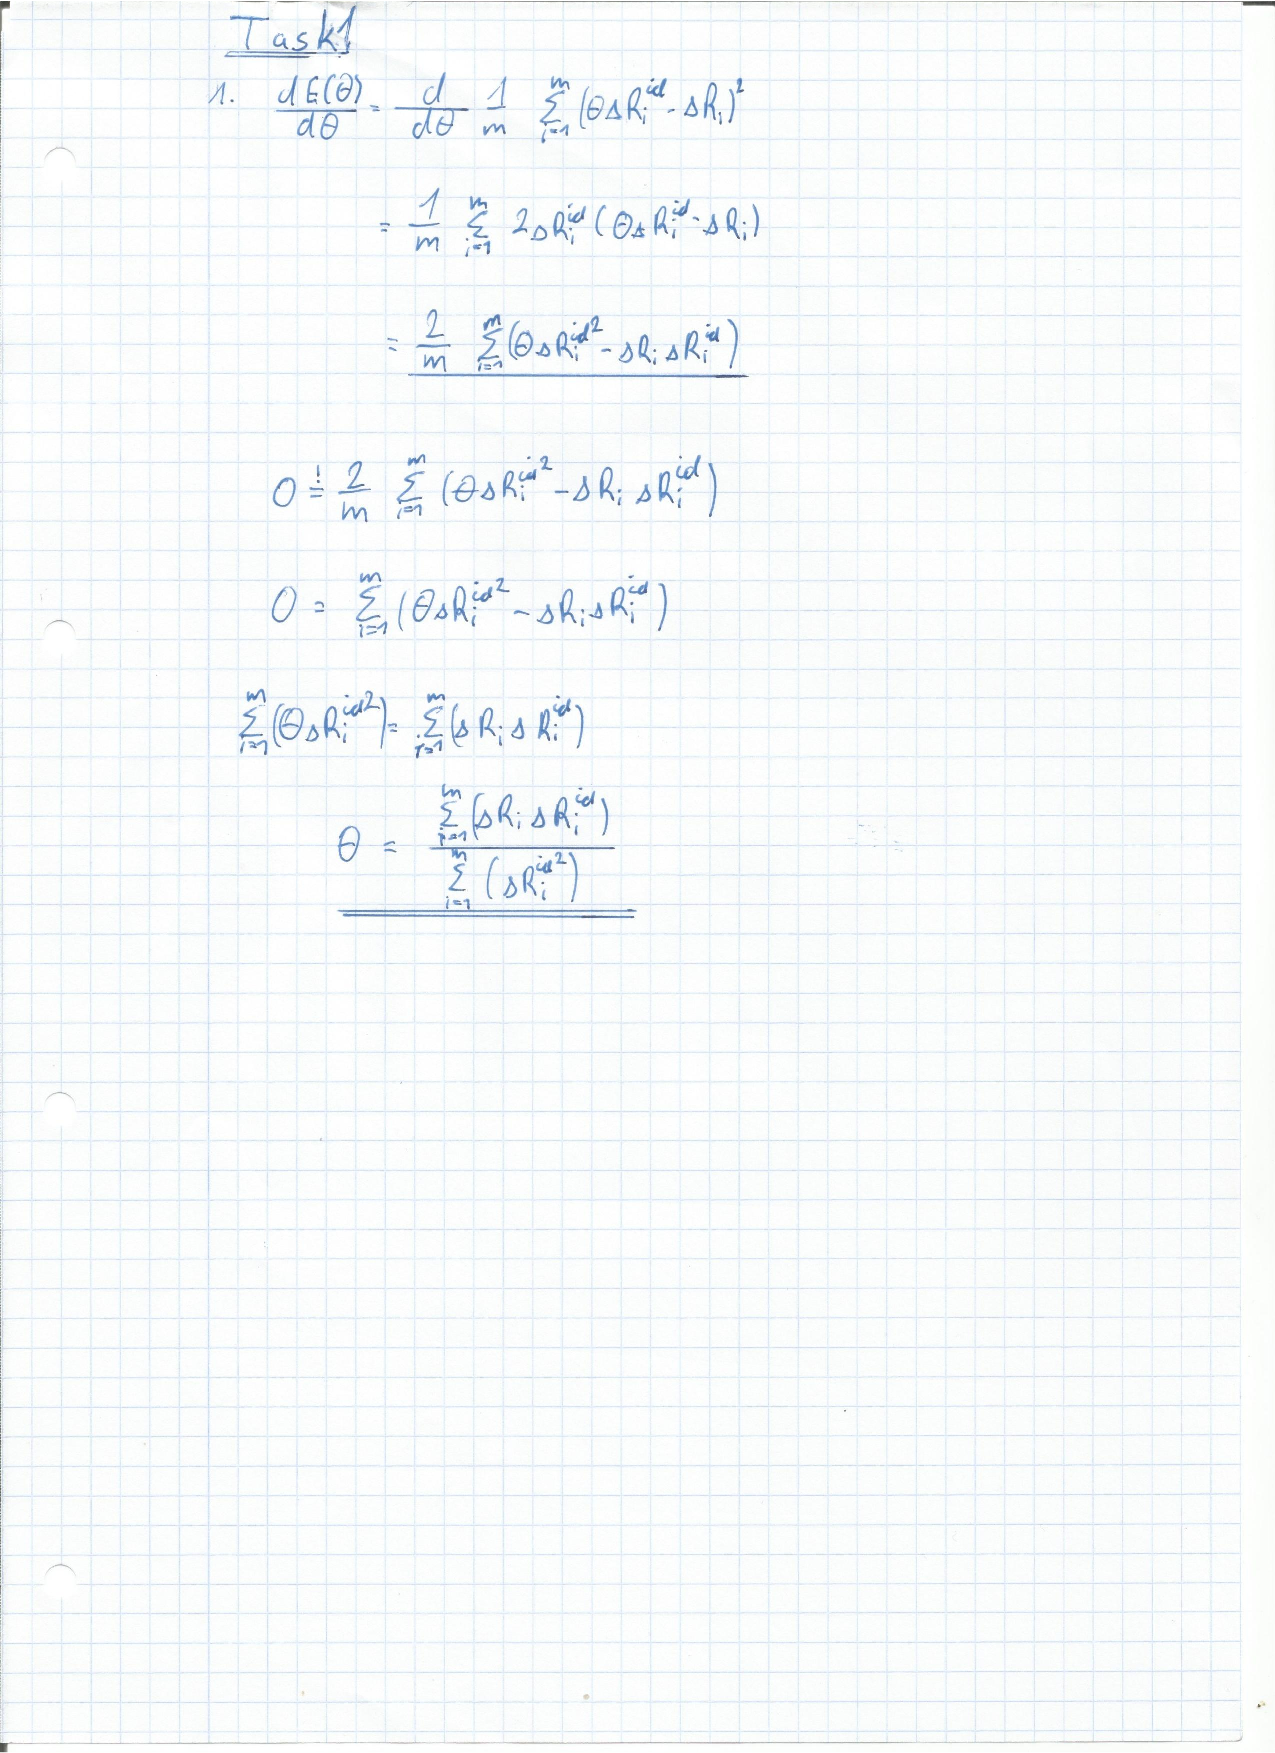
\includepdf[pages={1-3}]{task1pnp}

    \subsection*{1.5 Results}
    \textbf{Model 1:} \\
    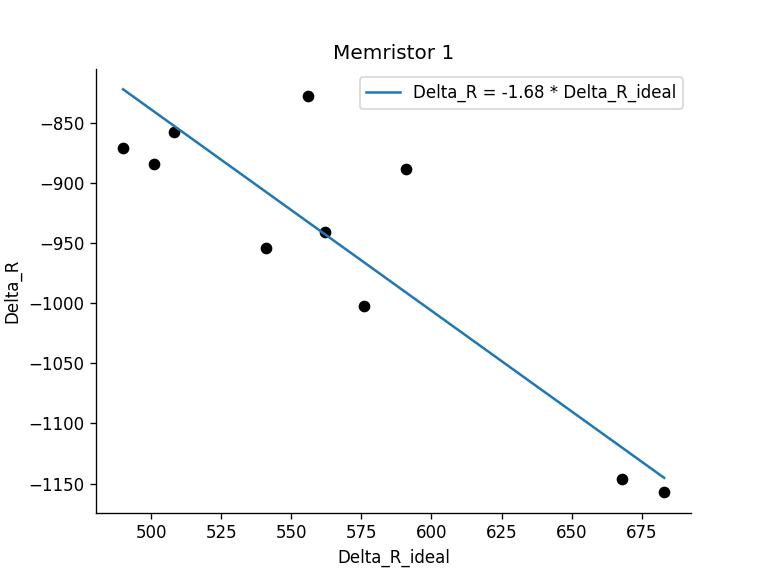
\includegraphics[width=\textwidth / 2]{code/plots/model_1_memristor_1}
    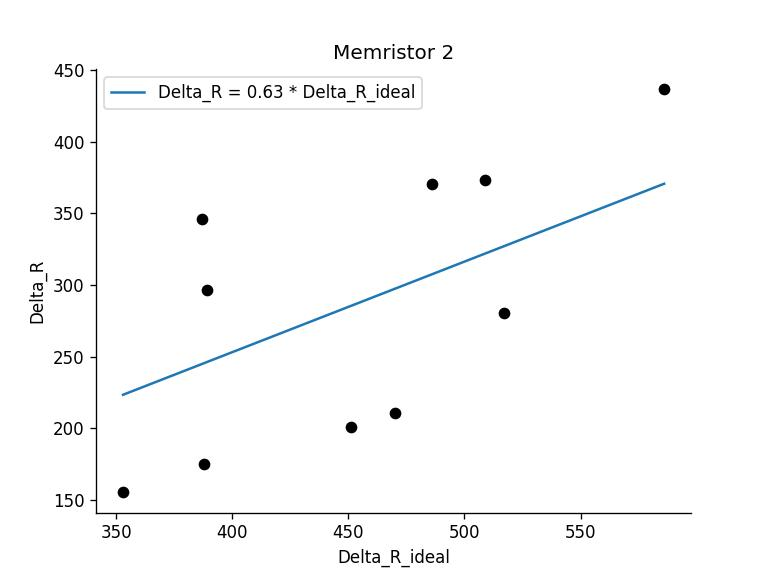
\includegraphics[width=\textwidth / 2]{code/plots/model_1_memristor_2}
    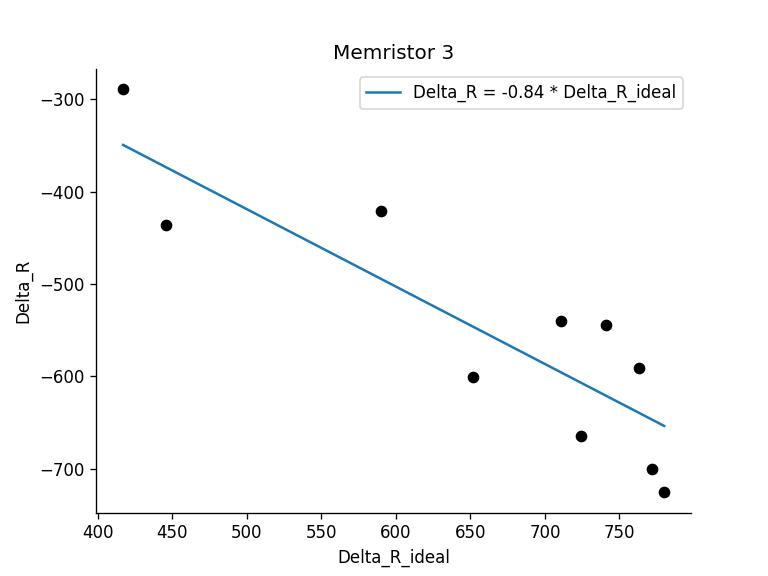
\includegraphics[width=\textwidth / 2]{code/plots/model_1_memristor_3}
    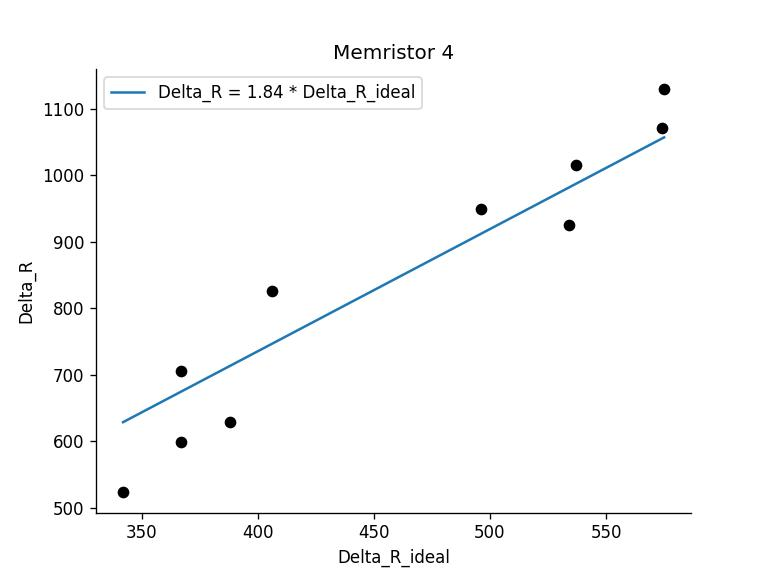
\includegraphics[width=\textwidth / 2]{code/plots/model_1_memristor_4}
    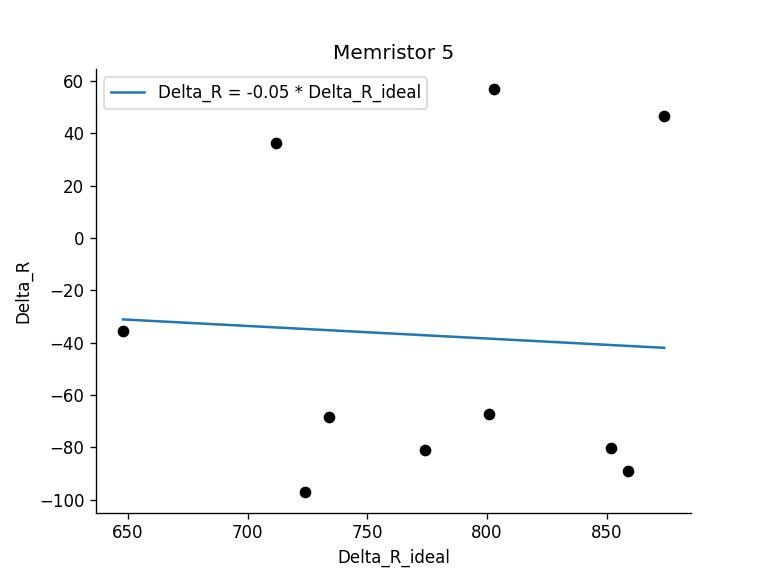
\includegraphics[width=\textwidth / 2]{code/plots/model_1_memristor_5}
    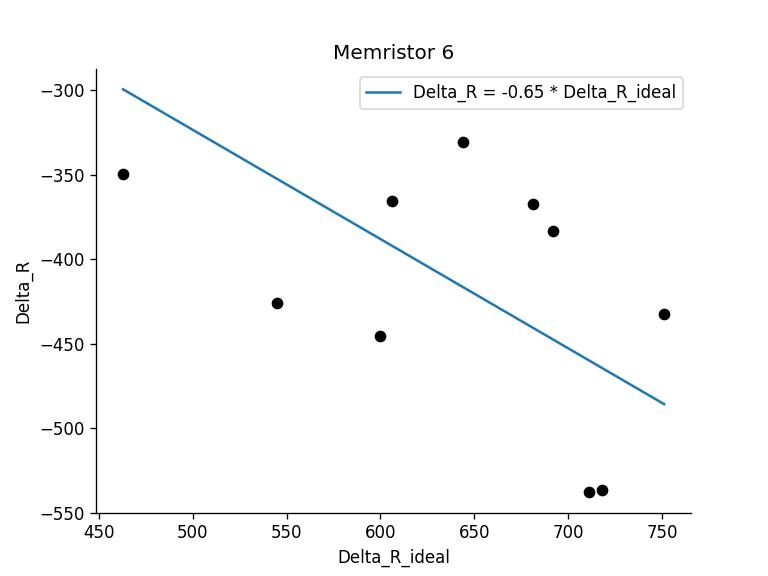
\includegraphics[width=\textwidth / 2]{code/plots/model_1_memristor_6}
    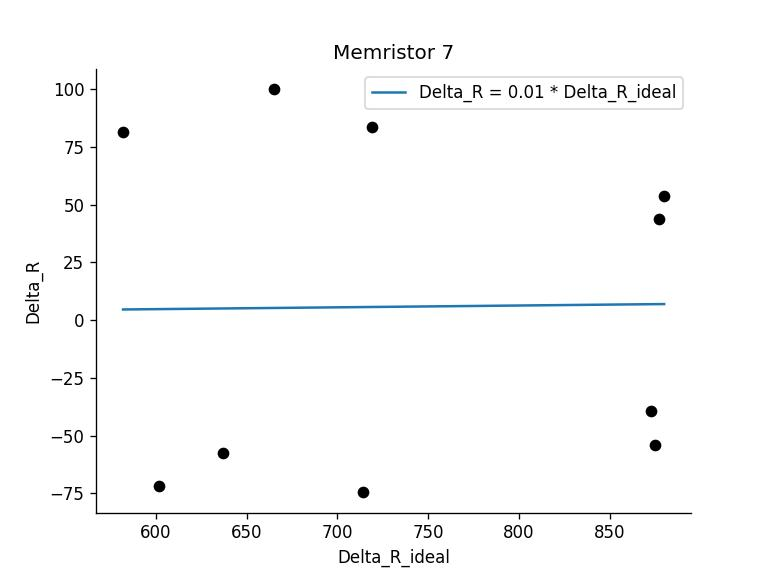
\includegraphics[width=\textwidth / 2]{code/plots/model_1_memristor_7}
    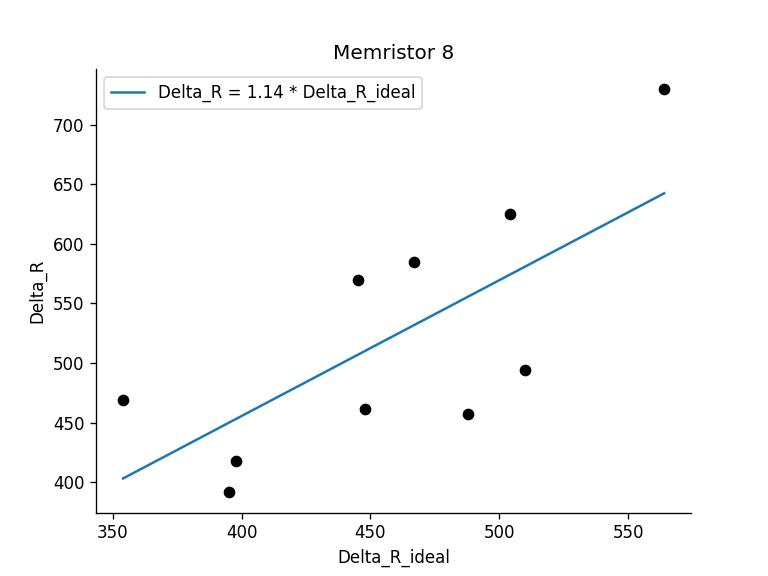
\includegraphics[width=\textwidth / 2]{code/plots/model_1_memristor_8}

    \pagebreak
    \textbf{Model 2} \\
    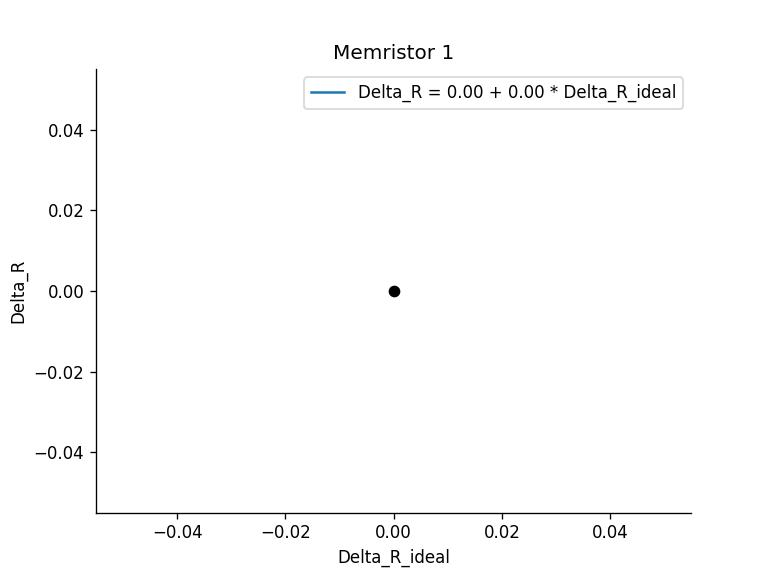
\includegraphics[width=\textwidth / 2]{code/plots/model_2_memristor_1}
    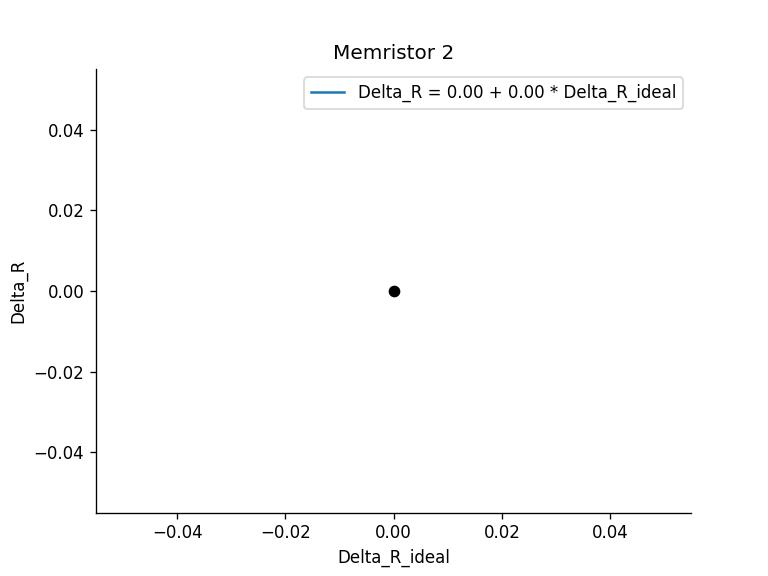
\includegraphics[width=\textwidth / 2]{code/plots/model_2_memristor_2}
    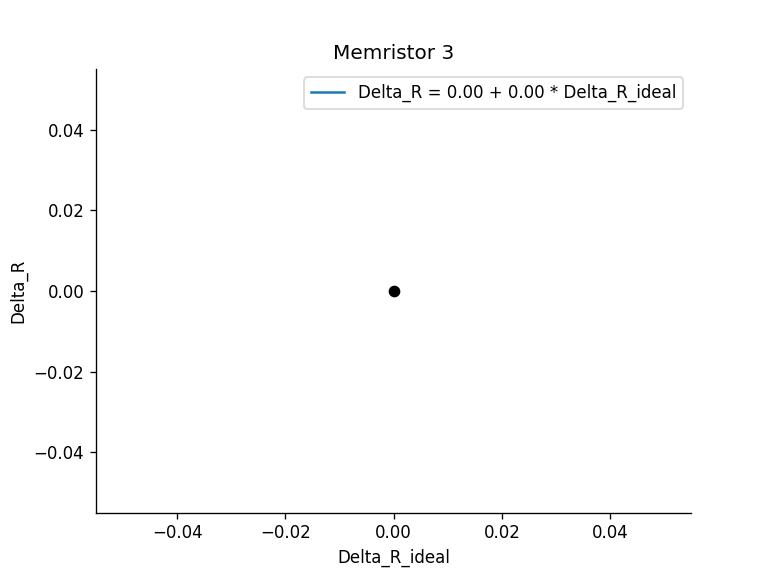
\includegraphics[width=\textwidth / 2]{code/plots/model_2_memristor_3}
    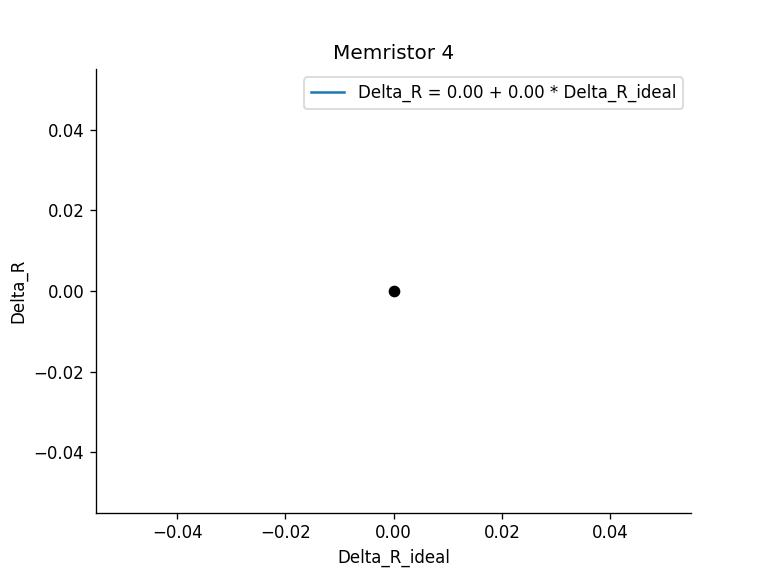
\includegraphics[width=\textwidth / 2]{code/plots/model_2_memristor_4}
    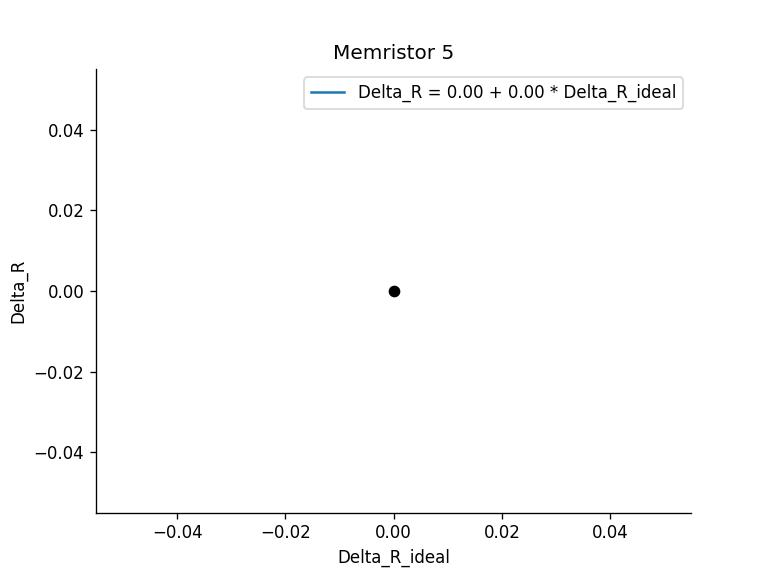
\includegraphics[width=\textwidth / 2]{code/plots/model_2_memristor_5}
    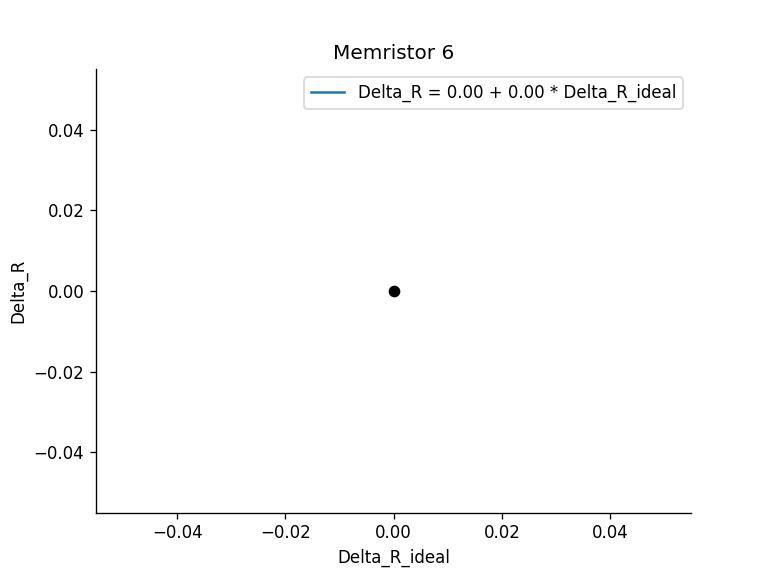
\includegraphics[width=\textwidth / 2]{code/plots/model_2_memristor_6}
    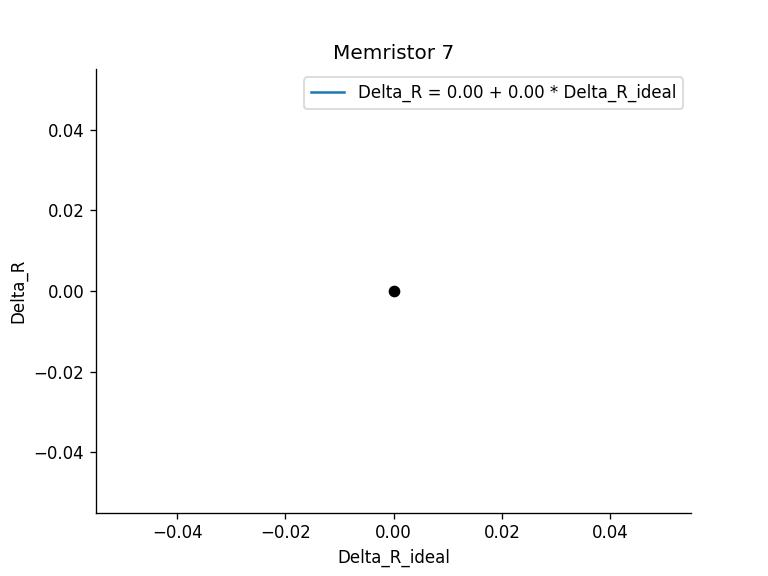
\includegraphics[width=\textwidth / 2]{code/plots/model_2_memristor_7}
    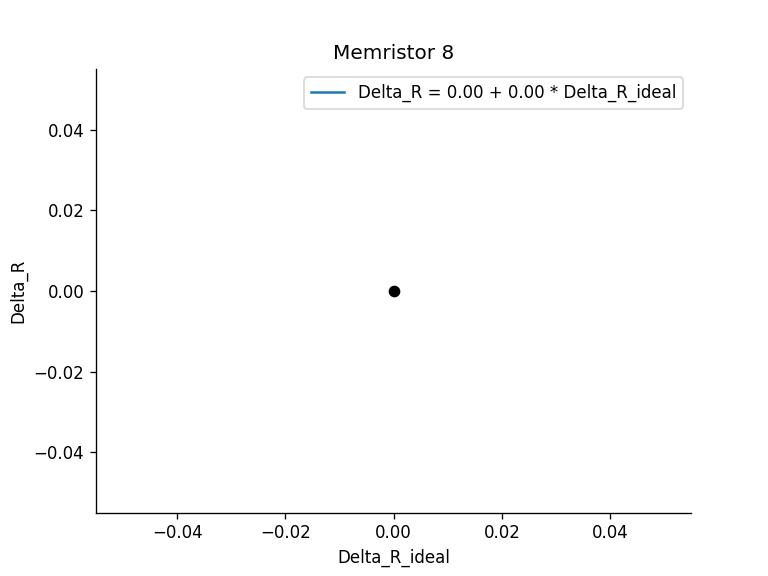
\includegraphics[width=\textwidth / 2]{code/plots/model_2_memristor_8}
    \pagebreak

    \subsection*{1.6 Interpretation}
    In Model 1, we can clearly see the effect of the parameter $\theta$.
    A positive $\theta$ produces an increasing slope, which correlates to a concordant fault.
    Similarly, a negative $\theta$ corresponds to a discordant fault,
    and a $\theta$ which is nearly zero corresponds to a stuck fault.

    Model 2 shows almost exactly the same results as Model 1.
    One can read the type of fault from parameter $\theta_1$ the same way as with $\theta$ in Model 1.
    The newly added intercept parameter shows a spontaneous change in resistance when $\Delta R^{ideal}$ is 0.

    \subsection*{1.7 Model choice}
    Though no big differences can be observed between the two models, Model 2 is slightly more accurate.
    This is because the added degree of freedom for the intercept lets is model faults more accurately,
    particularly if a memristor drifts in resistance spontaneously.
    This can be seen most prominently in Memristor 4.

    \subsection*{1.8 Identifying faults}
    This piece of code was added to interpret the type of fault.
    If the absolute value of $\theta_1$ is below $0.1$, it is classified as a stuck fault.
    Otherwise, if it is positive, it is a concordant fault, else it is a discordant fault.
    \begin{lstlisting}
        for i in range(n_memristor):
            print("Memristor %d: %s fault" % (
                i,
                "stuck" if abs(thetas[i][1]) < 0.1 else \
                  ("concordant" if thetas[i][1] > 0 else "discordant")
            ))
    \end{lstlisting}
    The output from the snippet was the following:
    \begin{lstlisting}
        Memristor 0: discordant fault
        Memristor 1: concordant fault
        Memristor 2: discordant fault
        Memristor 3: concordant fault
        Memristor 4: stuck fault
        Memristor 5: discordant fault
        Memristor 6: stuck fault
        Memristor 7: concordant fault
    \end{lstlisting}

    \subsection*{1.Bonus Testing}
    The test cases were engineered to show the limitations of Model 1,
    and to check that both Models were implemented correctly.
    Note that an Error of $10^{-10}$ was allowed to allow floating point errors.

    \begin{lstlisting}
    def test_fit_zero_intercept_lin_model():
        tests = np.array([
            [[100, 150], [200, 300], [300, 450], [400, 600]],
            [[100, -150], [200, -300], [300, -450], [400, -600]],
            [[100, 50], [100, -50], [200, 50], [200, -50]],
            [[100, 50], [100, 50], [200, 50], [200, 50]],
        ])
        correct_thetas = [1.5, -1.5, 0, 0.3]

        for i in range(len(correct_thetas)):
            x = tests[i, :, 0]
            y = tests[i, :, 1]
            theta = fit_zero_intercept_lin_model(x, y)
            assert(abs(theta - correct_thetas[i]) < 1e-10)
        return 0


    def test_fit_lin_model_with_intercept():
        tests = np.array([
            [[100, 150], [200, 300], [300, 450], [400, 600]],
            [[100, 250], [200, 400], [300, 550], [400, 700]],
            [[100, -150], [200, -300], [300, -450], [400, -600]],
            [[100, 150], [100, 50], [200, 150], [200, 50]],
            [[100, 50], [100, 50], [200, 50], [200, 50]],
        ])
        correct_thetas = [[0, 1.5], [100, 1.5], [0, -1.5], [100, 0], [50, 0]]

        for i in range(len(correct_thetas)):
            x = tests[i, :, 0]
            y = tests[i, :, 1]
            theta_0, theta_1 = fit_lin_model_with_intercept(x, y)
            assert(abs(theta_0 - correct_thetas[i][0]) < 1e-10)
            assert(abs(theta_1 - correct_thetas[i][1]) < 1e-10)
        return 0
    \end{lstlisting}

    \pagebreak
    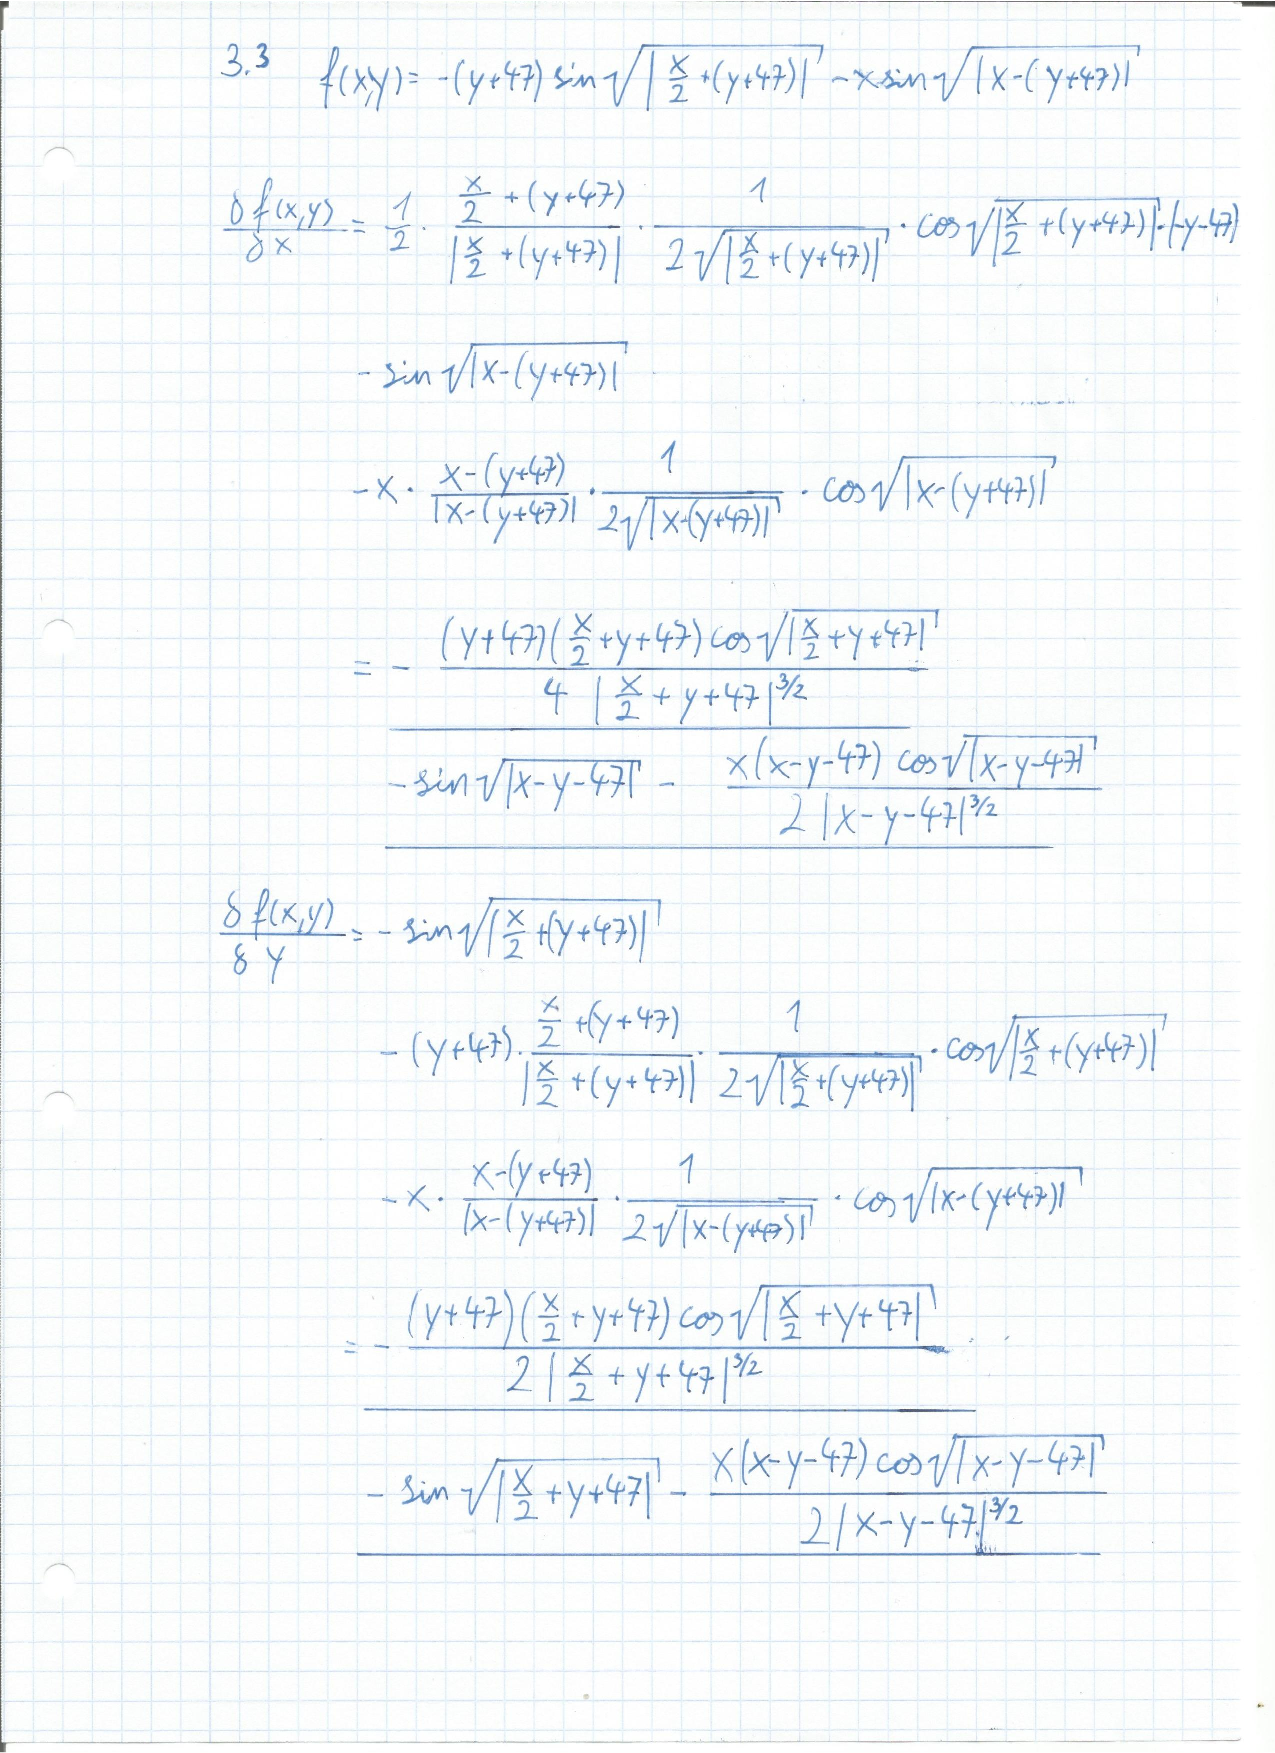
\includepdf{task3pnp}

    \subsection*{3.4 Convergence}
    The following graphs show the convergence rates with $10^{-4}$, $10^{-6}$ and $10^{-10}$ learning rate respectively.
    Note that none of the runs has converged on the true minimum of the function.\\
    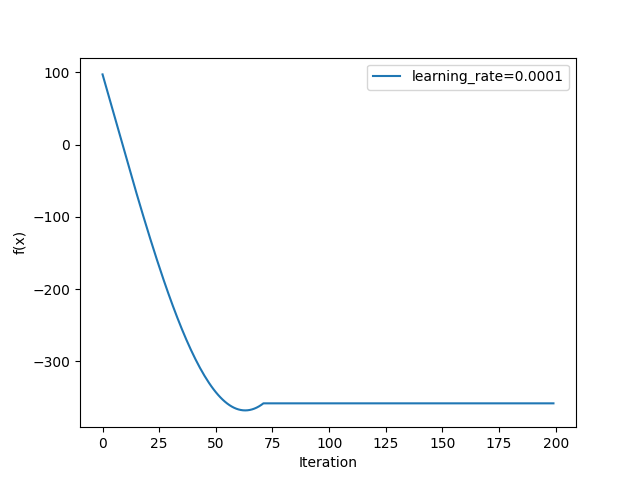
\includegraphics[width=\textwidth / 2]{3_fast_learn}
    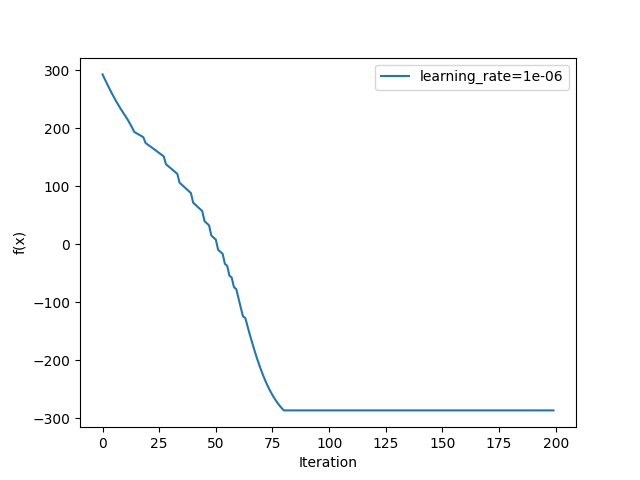
\includegraphics[width=\textwidth / 2]{3_mid_learn}
    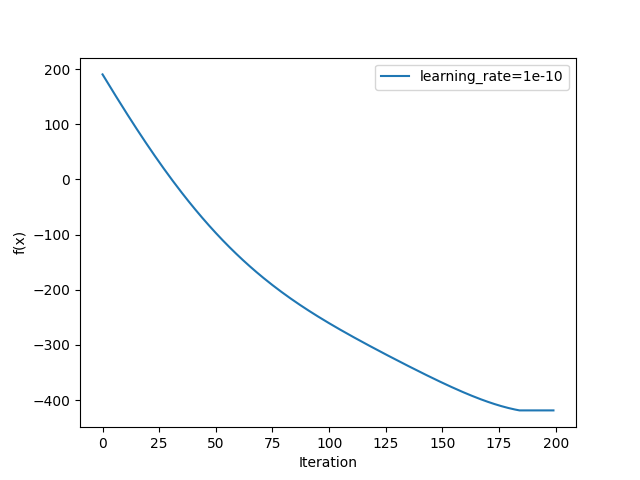
\includegraphics[width=\textwidth / 2]{3_slow_learn}

    \subsection*{3.5 Challenges}
    The function is hard to optimize because it has very many local minima.
    An optimizing algorithm easily gets stuck on one of these local minima, and never gets near the global minimum.
    As a result, the algorithm was never able to find the global minimum in our tests.

    \subsection*{3.6 Differentiability}
    The absolute function has a sharp point at location $0$.
    This means that there is no defined derivative of the function at this point.
    Another way to look at this is that the derivative of $|u|$ is $\frac{u}{|u|}$, which is undefined for $u = 0$.
    This makes optimisation even harder since an undefined derivative makes the descent step meaningless.
    
    \subsection*{3.7 Problematic points}
    The gradient of the Eggholder function might be problematic in points where the Eggholder function is not differentiable. To find these points 	we can take a look at the derivatives w.r.t. x and y and check if there are any points x,y where one of these derivatives is not defined. 
	Specifically, we take a look at the denominators in these derivatives. For certain points like (47, 0) or (48, 1) (these are the points we 			tested) this part of one denominator $\frac{x}{2} + y + 47$ will be zero which results in a division by zero, making these points problematic. 	Therefore, for the cases where the denominator might become zero, we add a small value to it to avoid an error and get an approximate result 		for the point.

\end{document}

%%%%%%%%% end snippet
